\documentclass{standalone}
\usepackage{tikz}
\usepackage{ctex,siunitx}
\setCJKmainfont{Noto Serif CJK SC}
\usepackage{tkz-euclide}
\usepackage{amsmath}
\usetikzlibrary{patterns, calc}
\usetikzlibrary {decorations.pathmorphing, decorations.pathreplacing, decorations.shapes,}
\begin{document}
\small
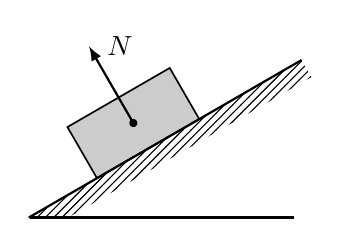
\begin{tikzpicture}[>=latex]
  % \useasboundingbox(-1,-0.75)rectangle(3.7,1.4);
  \draw [rotate=30, fill=black!20,semithick] (0,0) rectangle (1.5,.75);
  % \fill [rotate=30, pattern = north east lines] (-1,-.25) rectangle (3,0);
  \fill [rotate=30, pattern = north east lines] (-1,0)--++(-30:0.5)--(3,-0.25)--(3,0);
  \draw[rotate=30,thick] (-1,0)--(3,0);
  \fill[rotate=30] (.75,.375) circle[radius=1.5pt];
  \draw[rotate=30, ->,thick](.75,.375)--(.75,1.5)node[right=1mm]{$N$};
  % \node at (.25,1.75){$N$};
  \draw[thick](-.85,-.5)--(2.5,-.5);
  \end{tikzpicture}
\end{document}